\begin{huge}
\textbf{Crosswise Comparison Table}
\end{huge}
\\

\noindent The comparison table below summarizes 20 state-of-art cross-chain solutions, varying from protocols to platforms. The level of blockchain interoperability\footnotemark[1] is defined by Overledger develop team using the following notation:
\begin{itemize}
    \item 1-c-1: Two connected blockchains per time with a connector;
    \item N-c-N: Many connected blockchains per time with connectors;
    \item 1-1: Two connected blockchain connected per time without connector;
    \item N-N: Many connected blockchains per time without connectors.
\end{itemize}

\footnotetext[1]{This concept is adopted from Quant Overledger White paper\cite{verdian2018quant}}

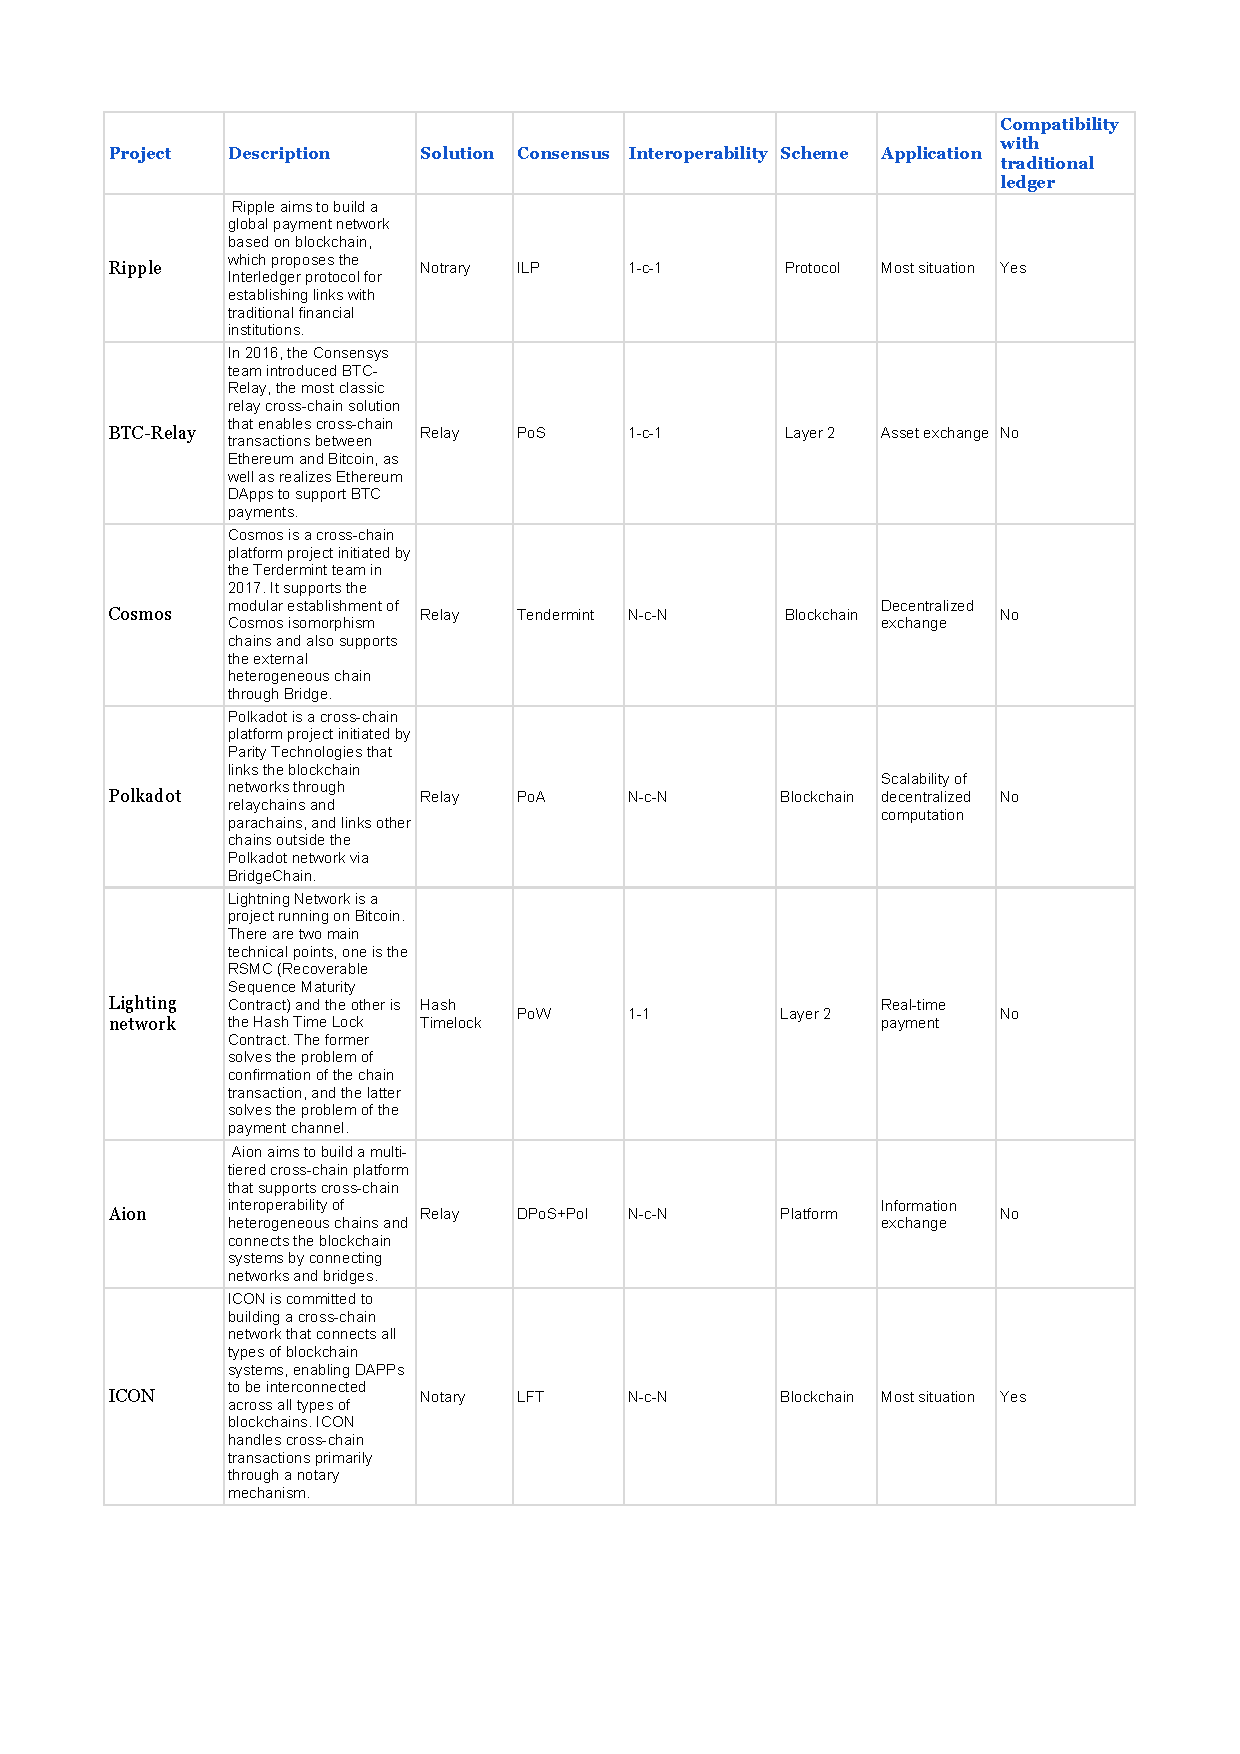
\includepdf[pages={1,2,3}]{table.pdf} 




